%! TEX program = pdflatex

\documentclass[oneside,solution]{tmpl}

\usepackage[utf8]{inputenc}
\usepackage[english,ukrainian]{babel}
\usepackage{float}

\title{Домашня робота}
\author{Захаров Дмитро}
\studentID{МП-31}
\instructor{Ігнатович С.Ю.}
\date{\today}
\duedate{23:59 30 квітня, 2024}
\assignno{8}
\semester{Весняний семестр 2024}
\mainproblem{Біфуркації}

\begin{document}

\maketitle

% \startsolution[print]

\problem{Система Лоренца.}

\hspace{20px}\textbf{Умова.} Дослідіть залежність характеру поведінки розв'язків системи Лоренца від значення параметрів. Наприклад, перевірити розрахунки, подані у Вікіпедії.

\textbf{Розв'язок.} Система Лоренца має наступний вигляд де $\boldsymbol{r} := (x,y,z)$:
\begin{equation}
    \dot{\boldsymbol{r}} = f(\boldsymbol{r}), \; 
    f(x,y,z) = 
    \begin{bmatrix}
        \sigma(y-x) \\
        x(\lambda - z) - y \\
        xy - bz
    \end{bmatrix}
\end{equation}

По суті, маємо параметризацію відносно параметрів $(\sigma,\lambda,b)$. Змінювати усі параметри разом дуже складно, тому зафіксуємо $\sigma=10,b=\frac{8}{3}$ і будемо змінювати $\lambda$. Також ми наведемо лінеаризацію системи і розрахунок стаціонарних точок, проте аналізувати Якобіан аналітично не будемо: насправді, це дуже об'ємна задача. Тому ми спробуємо дійсно перевірити результати з Вікіпедії, зобразивши систему у відповідних значеннях $\lambda$.

Отже, права частина система не є лінійною, оскільки містить доданки $xz$ та $xy$. Лінеаризація системи:
\begin{equation}
    \boldsymbol{J}(\boldsymbol{r})=\frac{\partial f}{\partial \boldsymbol{r}} = \begin{bmatrix}
        \frac{\partial f_x}{\partial x} & \frac{\partial f_x}{\partial y} & \frac{\partial f_x}{\partial z} \\
        \frac{\partial f_y}{\partial x} & \frac{\partial f_y}{\partial y} & \frac{\partial f_y}{\partial z} \\
        \frac{\partial f_z}{\partial x} & \frac{\partial f_z}{\partial y} & \frac{\partial f_z}{\partial z}
    \end{bmatrix} = \begin{bmatrix}
        -\sigma & \sigma & 0 \\
        \lambda - z & -1 & -x \\
        y & x & -b
    \end{bmatrix}
\end{equation}

Тепер знайдемо точки спокою. Для цього розв'язуємо систему:
\begin{equation}
    \begin{cases}
        \sigma(y-x) = 0 \\
        x(\lambda - z) - y = 0 \\
        xy - bz = 0
    \end{cases}
\end{equation}

З першого рівняння $x=y$, а тоді з третього $z = \frac{x^2}{b}$. Підставляючи у друге маємо $x\left(\lambda - \frac{x^2}{b}\right) - x = 0$. Очевидно, що один з розв'язків $\boldsymbol{r}=(0,0,0)$. Якщо ж $x \neq 0$, то маємо $\lambda - \frac{x^2}{b} = 1$, звідки $x^2 = b(\lambda - 1)$. Якщо $\lambda=1$, то маємо єдину точку спокою -- $(0,0,0)$. Інакше, якщо $\lambda>1$, то $x = \pm\sqrt{b(\lambda-1)}=y$, а тоді $z=\lambda-1$. Отже, при $\lambda > 1$, маємо три точки спокою:
\begin{gather}
    (0,0,0) \nonumber \\
    (\sqrt{b(\lambda-1)},\sqrt{b(\lambda-1)},\lambda-1) \nonumber \\
    (-\sqrt{b(\lambda-1)},-\sqrt{b(\lambda-1)},\lambda-1)
\end{gather}

Далі, розглядаємо випадки.

\textbf{Випадок 1.} $0 < \lambda < 1$. Маємо лише одну стаціонарну точку $(0,0,0)$ -- стійкий вузол, система стабільна.

\begin{figure}[H]
    \centering
    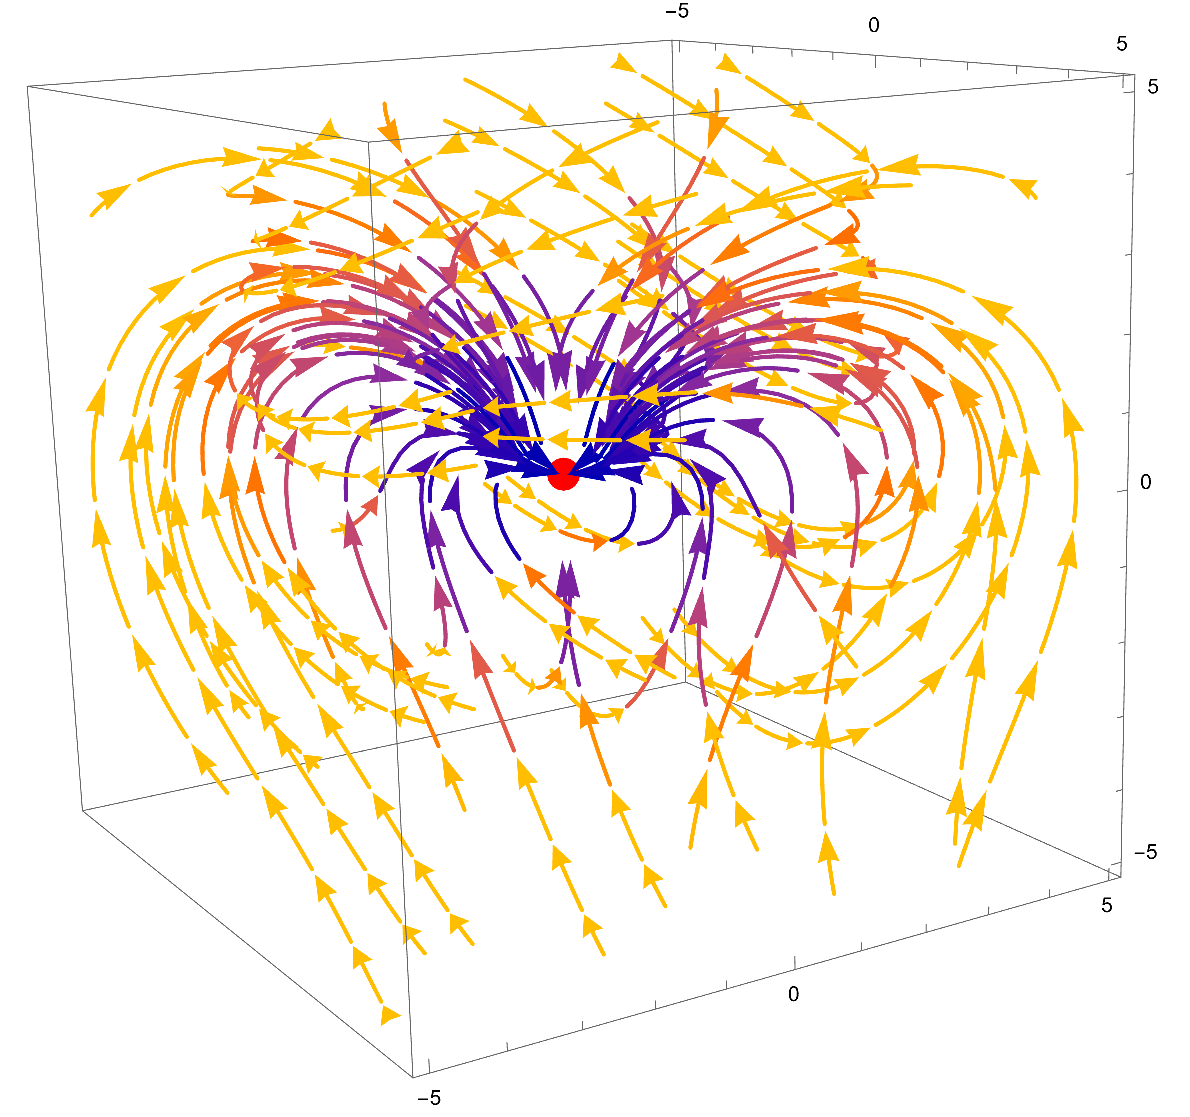
\includegraphics[width=0.75\textwidth]{images/hw_8/lorentz_case_1.pdf}
    \caption{Фазовий портрет системи при $\lambda = 0.5$.}
\end{figure}

\textbf{Випадок 2.} $1 < \lambda < 13.926$. Точка $(0,0,0)$ стає нестійкою, також з'являються дві нові точки спокою -- фокуси. Параметр $\lambda_1=13.926$ знаходиться чисельно і відповідає випадку, коли траєкторія, що почалася в $(0,0,0)$, повертається в нуль через деякий час.

\begin{figure}[H]
    \centering
    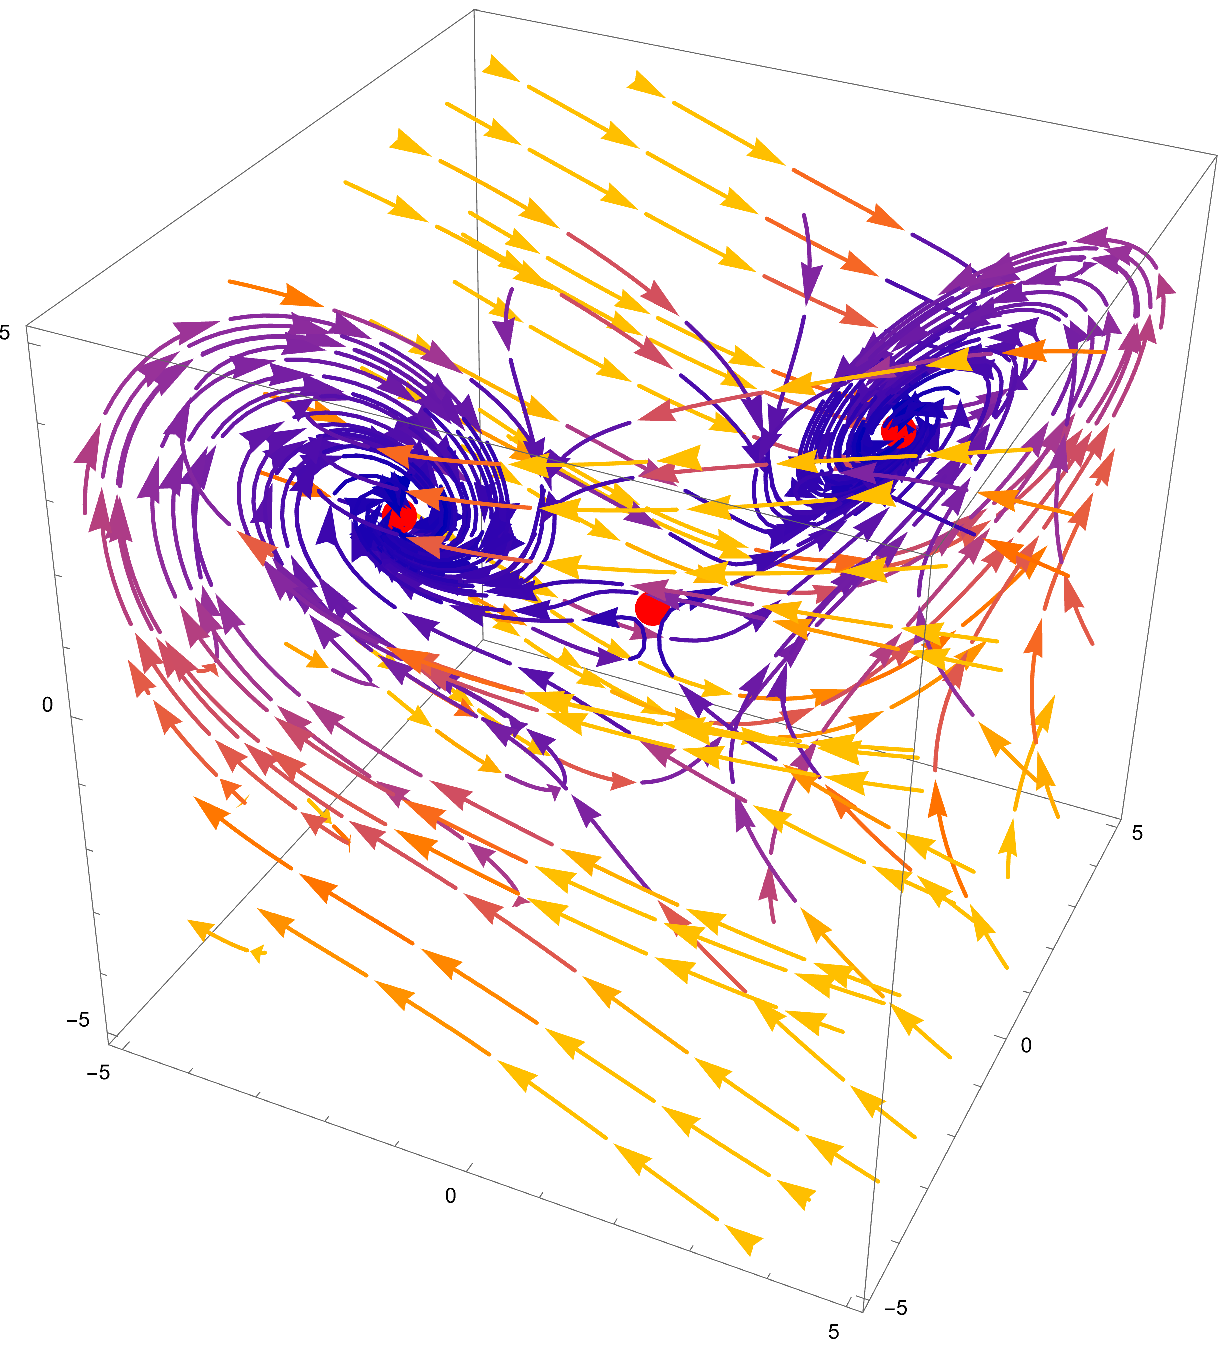
\includegraphics[width=0.75\textwidth]{images/hw_8/lorentz_case_2.pdf}
    \caption{Фазовий портрет системи при $\lambda = 3.0$.}
\end{figure}

\textbf{Випадок 3.} $13.926 < \lambda < 24$. $(0,0,0)$ і далі нестійка, а ось дві інші точки спокою набувають нестійкі граничні цикли навколо себе. Параметр $\lambda_2 \approx 24$ позначає, що далі стаціонарні точки втрачають стійкість\footnote{Насправді, у Вікіпедії наведений ще один відрізок після $\lambda_2$, але візуально вони у мене не сильно відрізняються.}.

\begin{figure}[H]
    \centering
    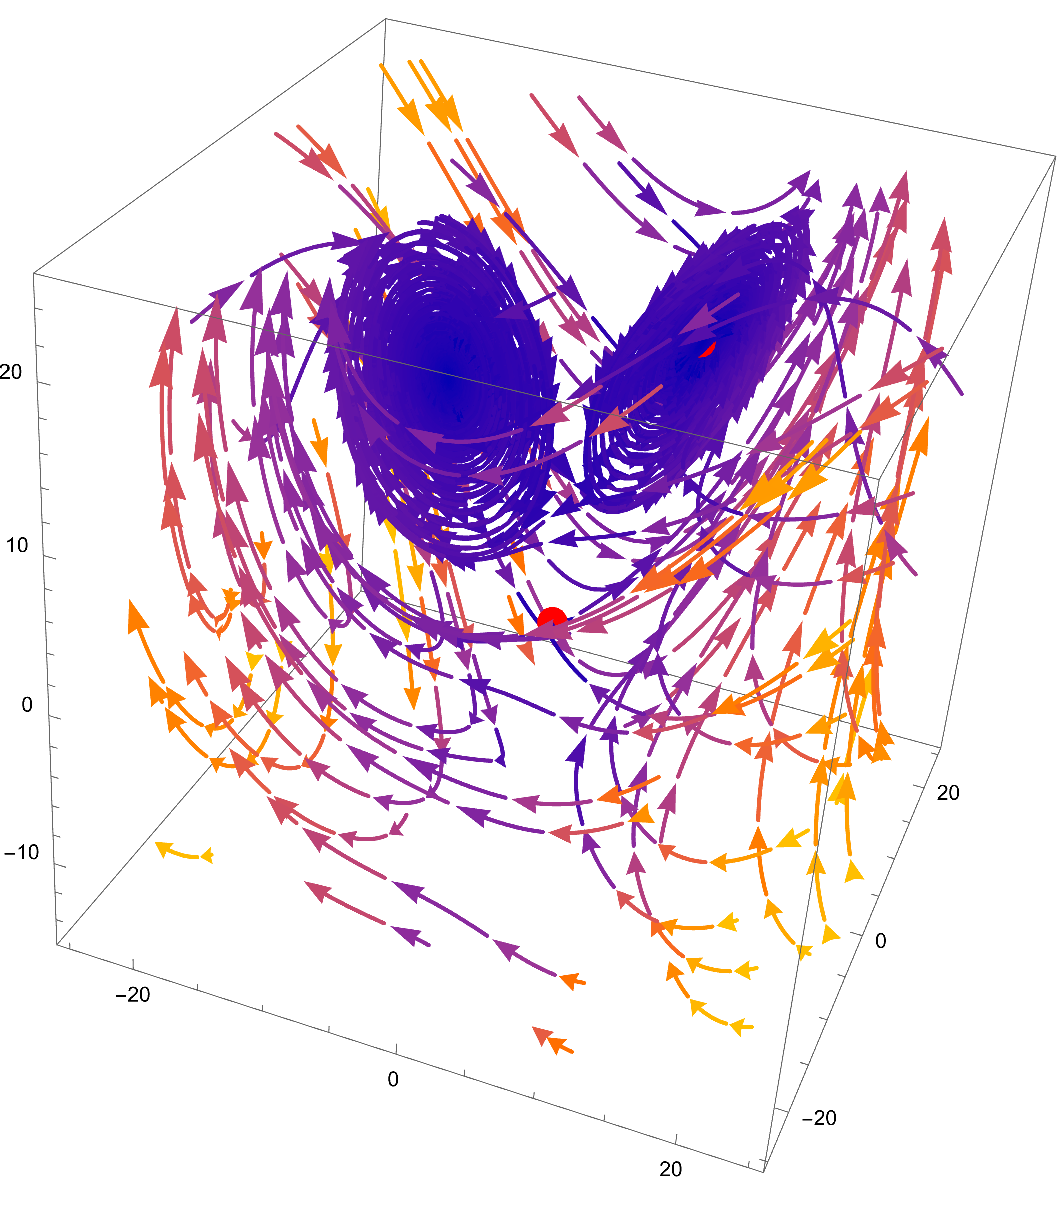
\includegraphics[width=0.75\textwidth]{images/hw_8/lorentz_case_3.pdf}
    \caption{Фазовий портрет системи при $\lambda = 18.0$.}
\end{figure}

\textbf{Випадок 4.} $\lambda > 24$. Стаціонарні точки втрачають стійкість і відбувається ефект дивного атрактора, коли точка може несподівано перестрибувати з однієї точки спокою на іншу.

\begin{figure}[H]
    \centering
    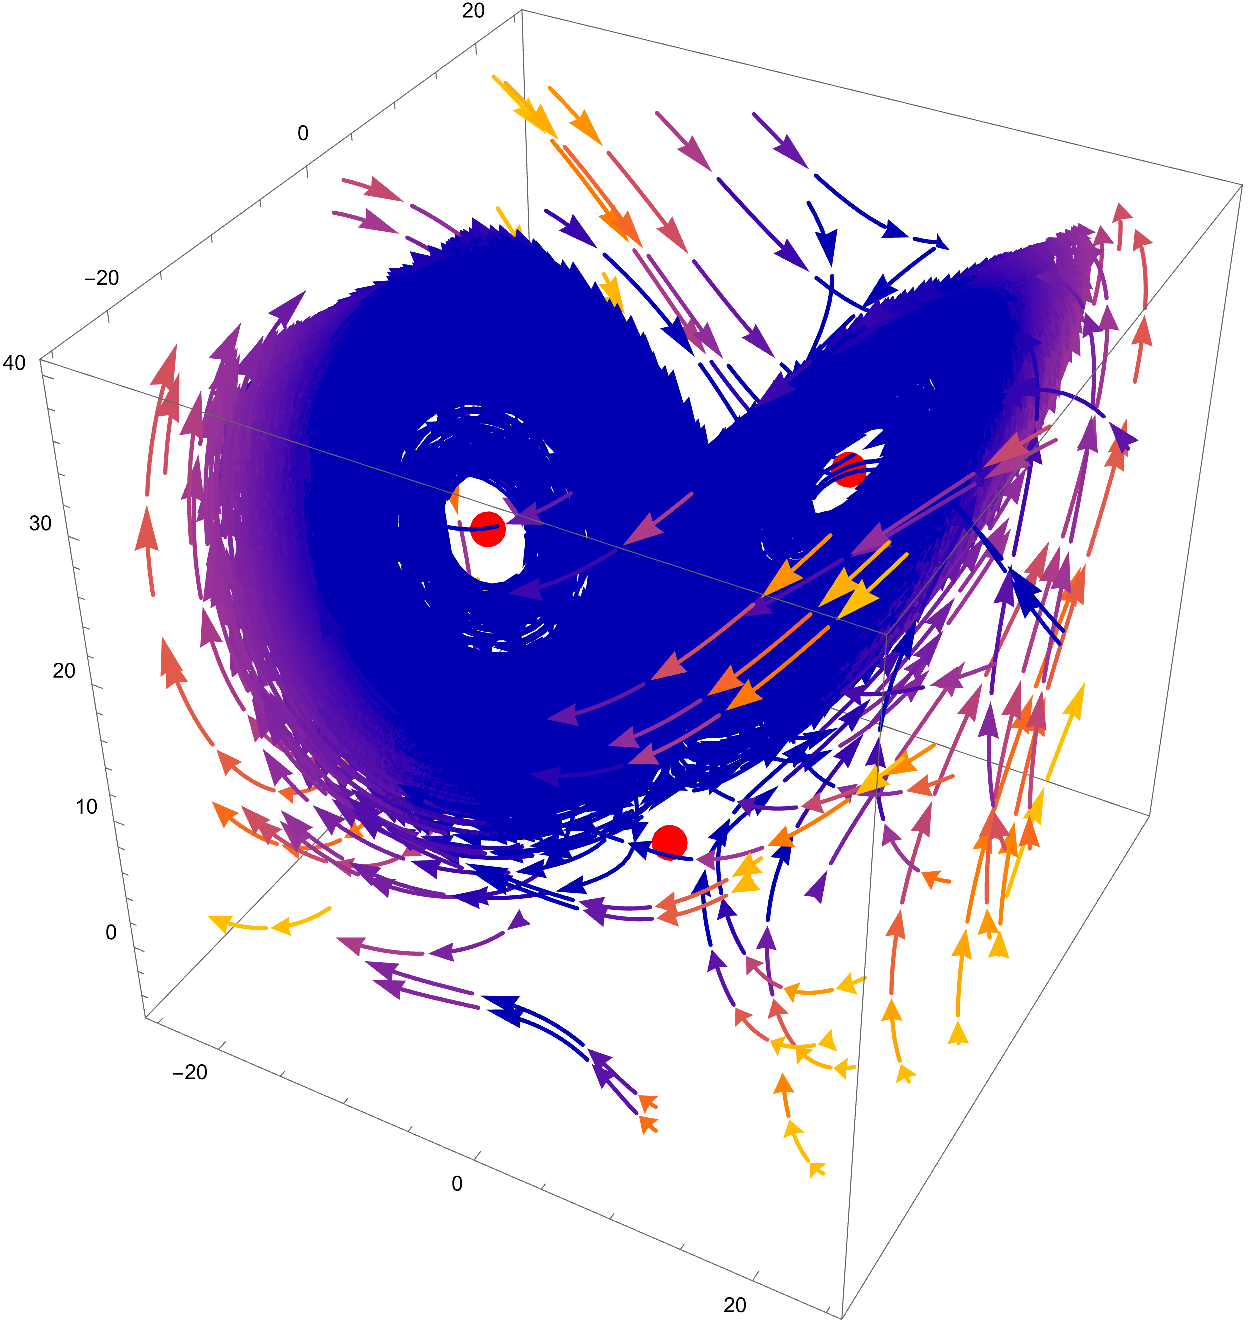
\includegraphics[width=0.75\textwidth]{images/hw_8/lorentz_case_4.pdf}
    \caption{Фазовий портрет системи при $\lambda = 27.0$.}
\end{figure}
\pagebreak
\problem{Класифікація портретів в $\mathbb{R}^3$.}

\hspace{20px}\textbf{Умова.} Для лінійних тривимірних систем $\dot{\mathbf{x}} = \boldsymbol{A}\mathbf{x}$ існує 10 ``грубих'' варіантів розташування власних значень матриці $\boldsymbol{A}$ на комплексній площині (які не змінюються при малих ворушіннях матриці): п'ять з них схематично зображені нижче, і ще п'ять симетричні поданим відносно уявної вісі.

\begin{figure}[H]
    \centering
    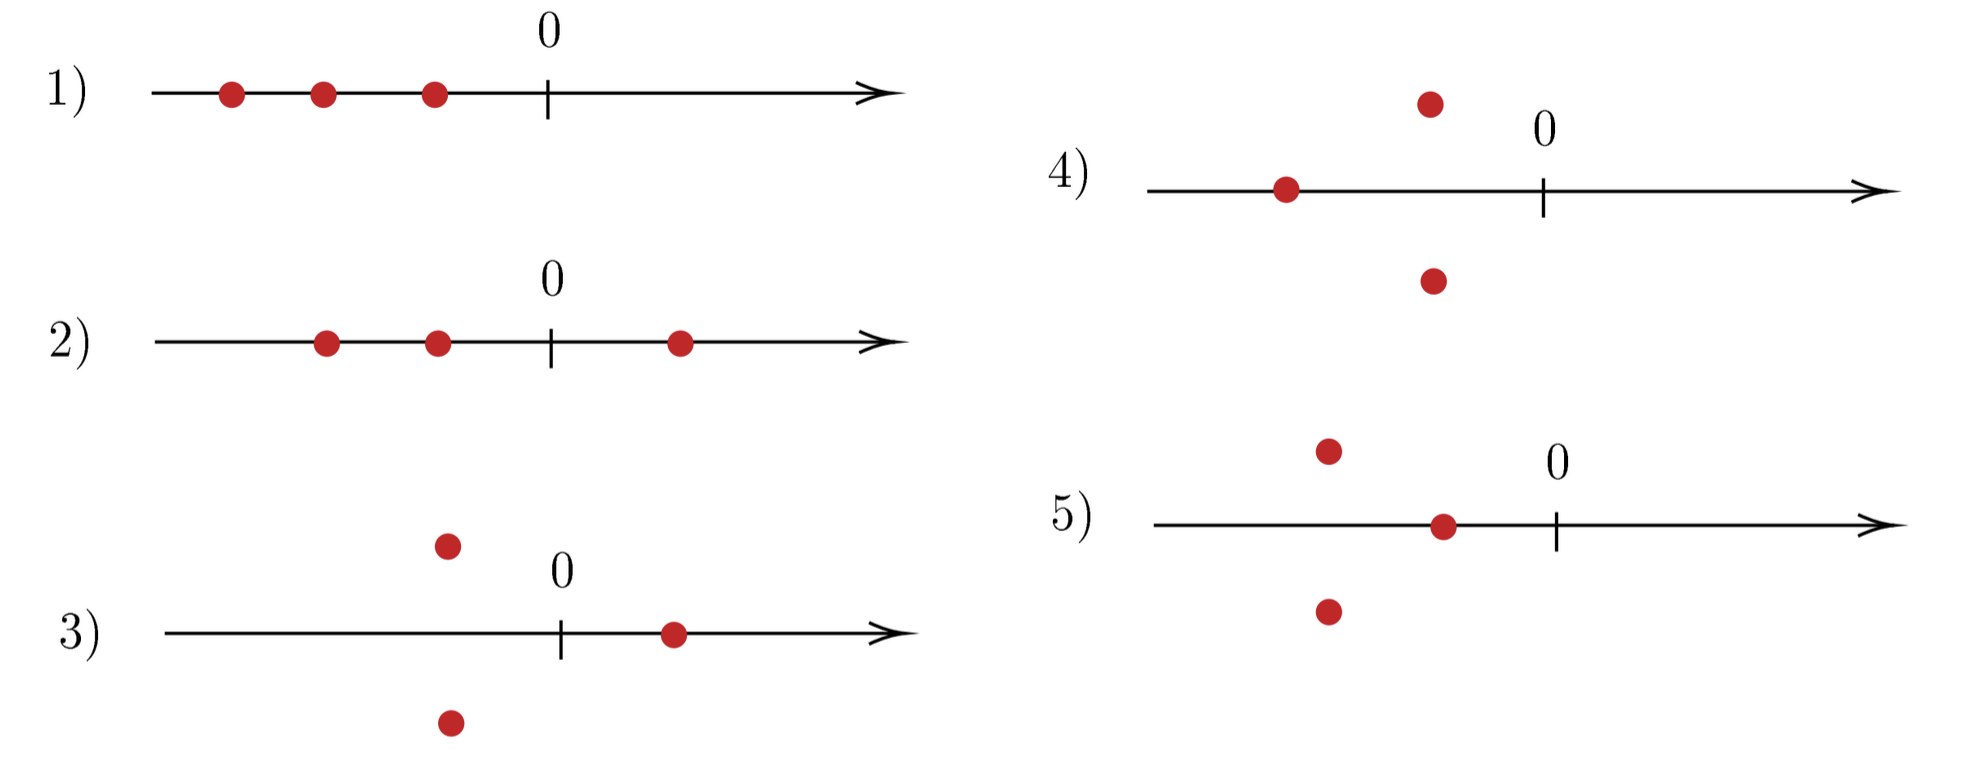
\includegraphics[width=\textwidth]{images/hw_8/problem_2_statement.png}
\end{figure}

Спробуйте намалювати ескізи фазових портретів систем з такими матрицями (у тривимірному просторі) або хоча б сформулювати, чим вони відрізняються один від одного.

\textbf{Розв'язок.} Отже, розглянемо кожен з випадків.

\textbf{Випадок 1.} $\lambda_1, \lambda_2,\lambda_3 < 0$. В такому випадку існує така зміна базису, в якій система набуває вигляд
\begin{equation}
    \begin{cases}
    \dot{y}_1 = \lambda_1 y_1 \\
    \dot{y}_2 = \lambda_2 y_2 \\
    \dot{y}_3 = \lambda_3 y_3
    \end{cases}
\end{equation}

Найлегше окремо розв'язати кожну систему. Маємо тоді параметризовану криву:
\begin{equation}
    \mathbf{y}(t) = (A_1 e^{\lambda_1 t}, A_2 e^{\lambda_2 t}, A_3 e^{\lambda_3 t})
\end{equation}

Помітимо, що $\lim_{t \to \infty}\mathbf{y}(t) = \mathbf{0}$, оскільки усі $\lambda_i < 0$. Тому, маємо щось накшталт стійкового вузлу, оскільки все сімейство кривих буде прямувати до початку координат (дивись рисунок нижче). 

\begin{figure}[H]
    \centering
    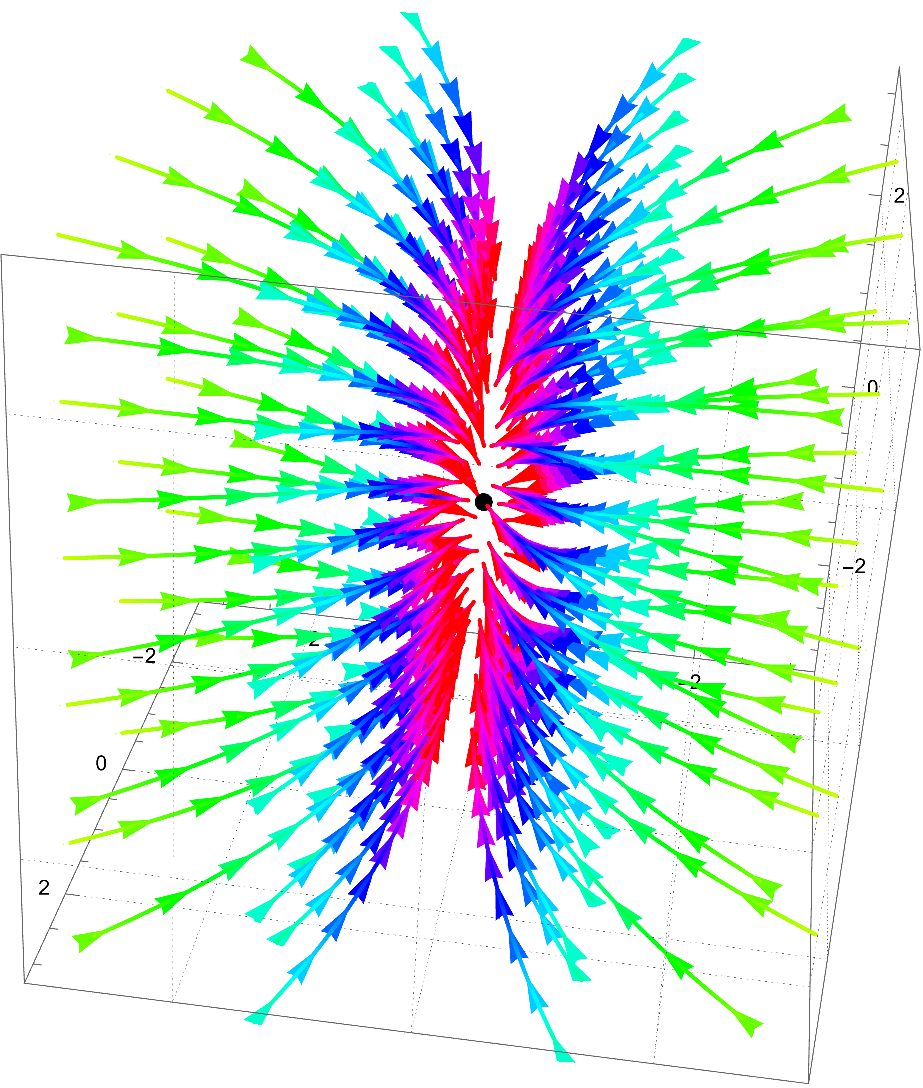
\includegraphics[width=0.5\textwidth]{images/hw_8/case_1.pdf}
\end{figure}

\textbf{Випадок 2.} $\lambda_1, \lambda_2 < 0, \; \lambda_3 > 0$. Це так само буде відповідати розв'язку
\begin{equation}
    \mathbf{y}(t) = (A_1e^{\lambda_1 t}, A_2e^{\lambda_2 t}, A_3e^{\lambda_3 t})
\end{equation}

Проте, в цьому випадку $\lim_{t \to \infty}y_1(t) = \lim_{t \to \infty}y_2(t) = 0$ -- проєкція на вісь $Oxy$ буде прямувати до $0$, але по вісі $Oz$ точка буде віддалятись. Це дуже схоже на випадок сідла. 
\begin{figure}[H]
    \centering
    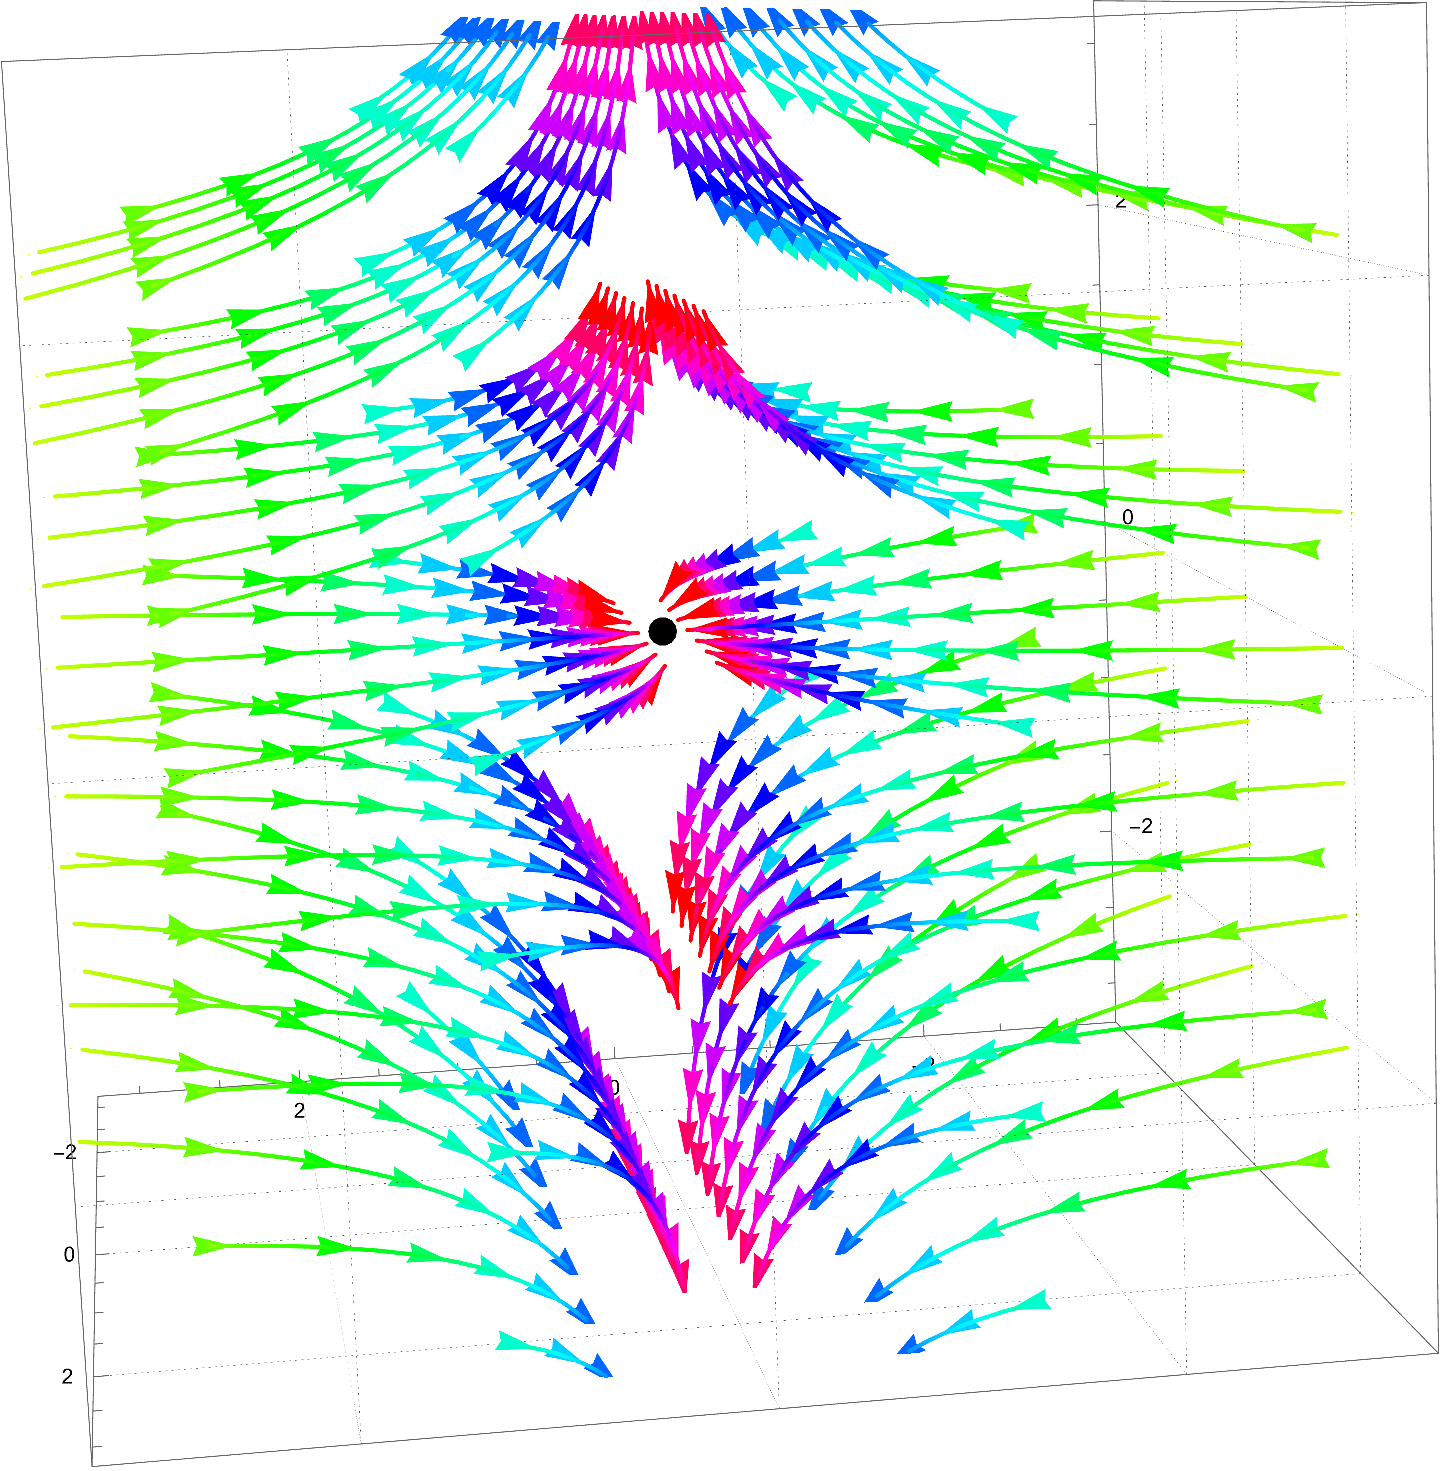
\includegraphics[width=0.5\textwidth]{images/hw_8/case_2.pdf}
\end{figure}

\textbf{Випадок 3.} $\lambda_1 = \lambda_2^*, \; \text{Re}(\lambda_1)<0, \; \lambda_3 > 0$. Тоді якщо $\lambda_1 = a+ib$, то систему можна звести до вигляду:
\begin{equation}
    \begin{cases}
        \dot{y}_1 = ay_1 + by_2 \\
        \dot{y}_2 = -by_1 + ay_2 \\
        \dot{y}_3 = \lambda_3 y_3
    \end{cases}
\end{equation}

Розв'язок перших двох рівнянь ми вже наводили у випадку двовимірної системи (точніше, у полярній формі, але запишемо її у координатній):
\begin{equation}
    (y_1(t),y_2(t)) = (C_1e^{at}\cos bt + C_2e^{at}\sin bt, C_2e^{at}\cos bt - C_1e^{at}\sin bt),
\end{equation}
що відповідала фокусу -- спіралі, що розкручується. У трьохвимірному випадку у якості третьої компоненти додаємо $C_3e^{\lambda_3t}, \lambda_3 > 0$. Маємо також щось накшталт фокусу, причому нестійкого (див. рис. 3).
\begin{figure}[H]
    \centering
    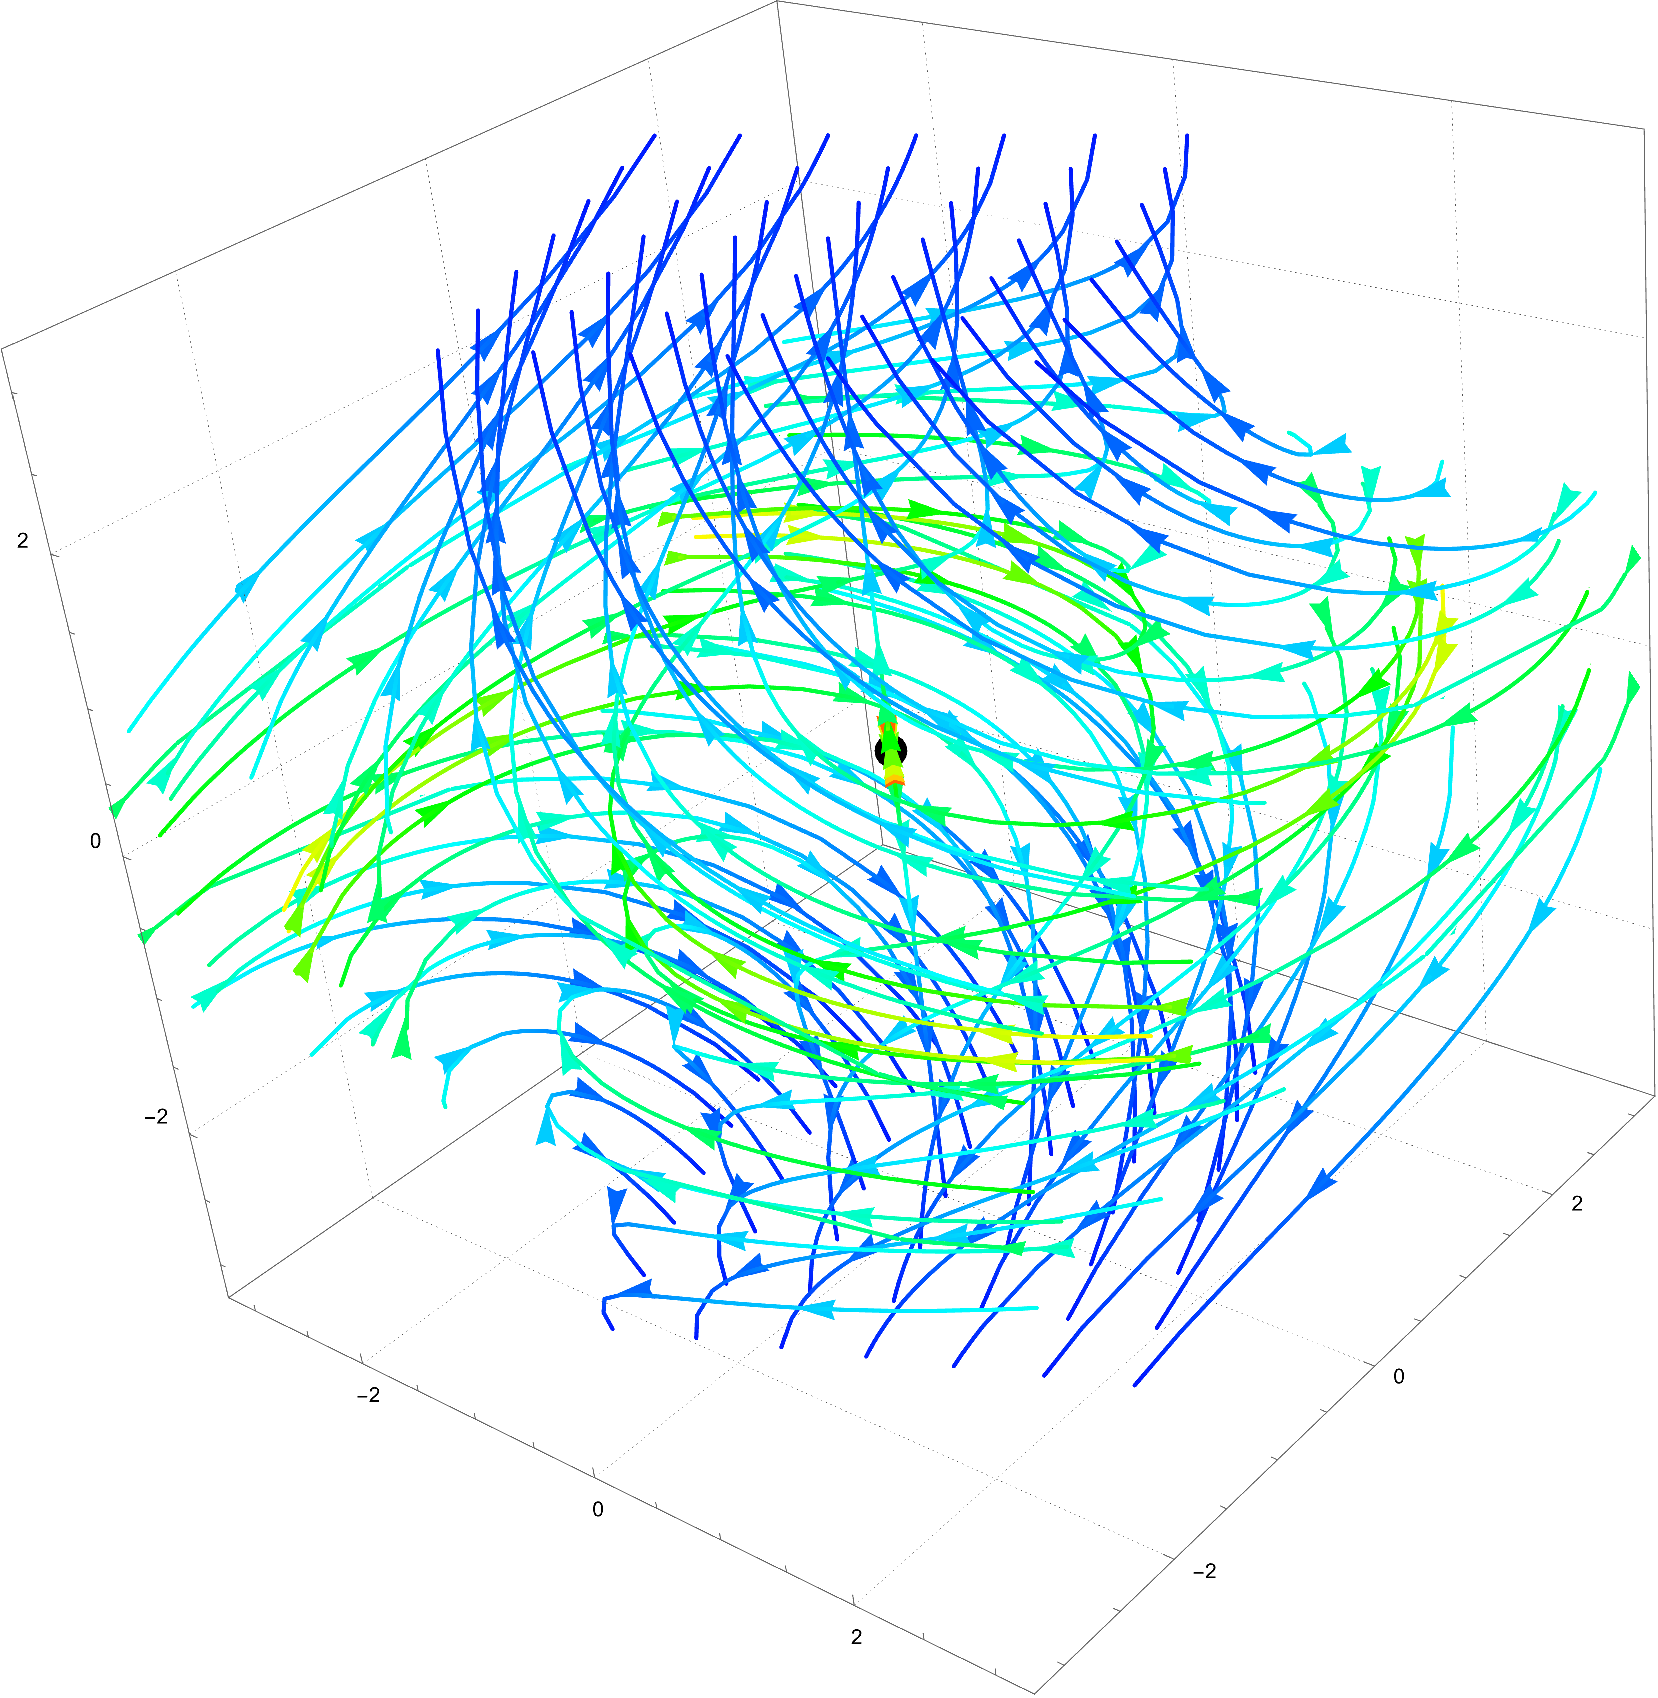
\includegraphics[width=0.5\textwidth]{images/hw_8/case_3.pdf}
\end{figure}

\textbf{Випадок 4.} $\lambda_1 = \lambda_2^*, \; \text{Re}(\lambda_1)<0, \; \lambda_3<\text{Re}(\lambda_1)$. По формулі маємо ту саму криву, як в випадку 3, лише за умови $\lambda_3 < 0$. Це буде відповідати стійкому фокусу.
\begin{figure}[H]
    \centering
    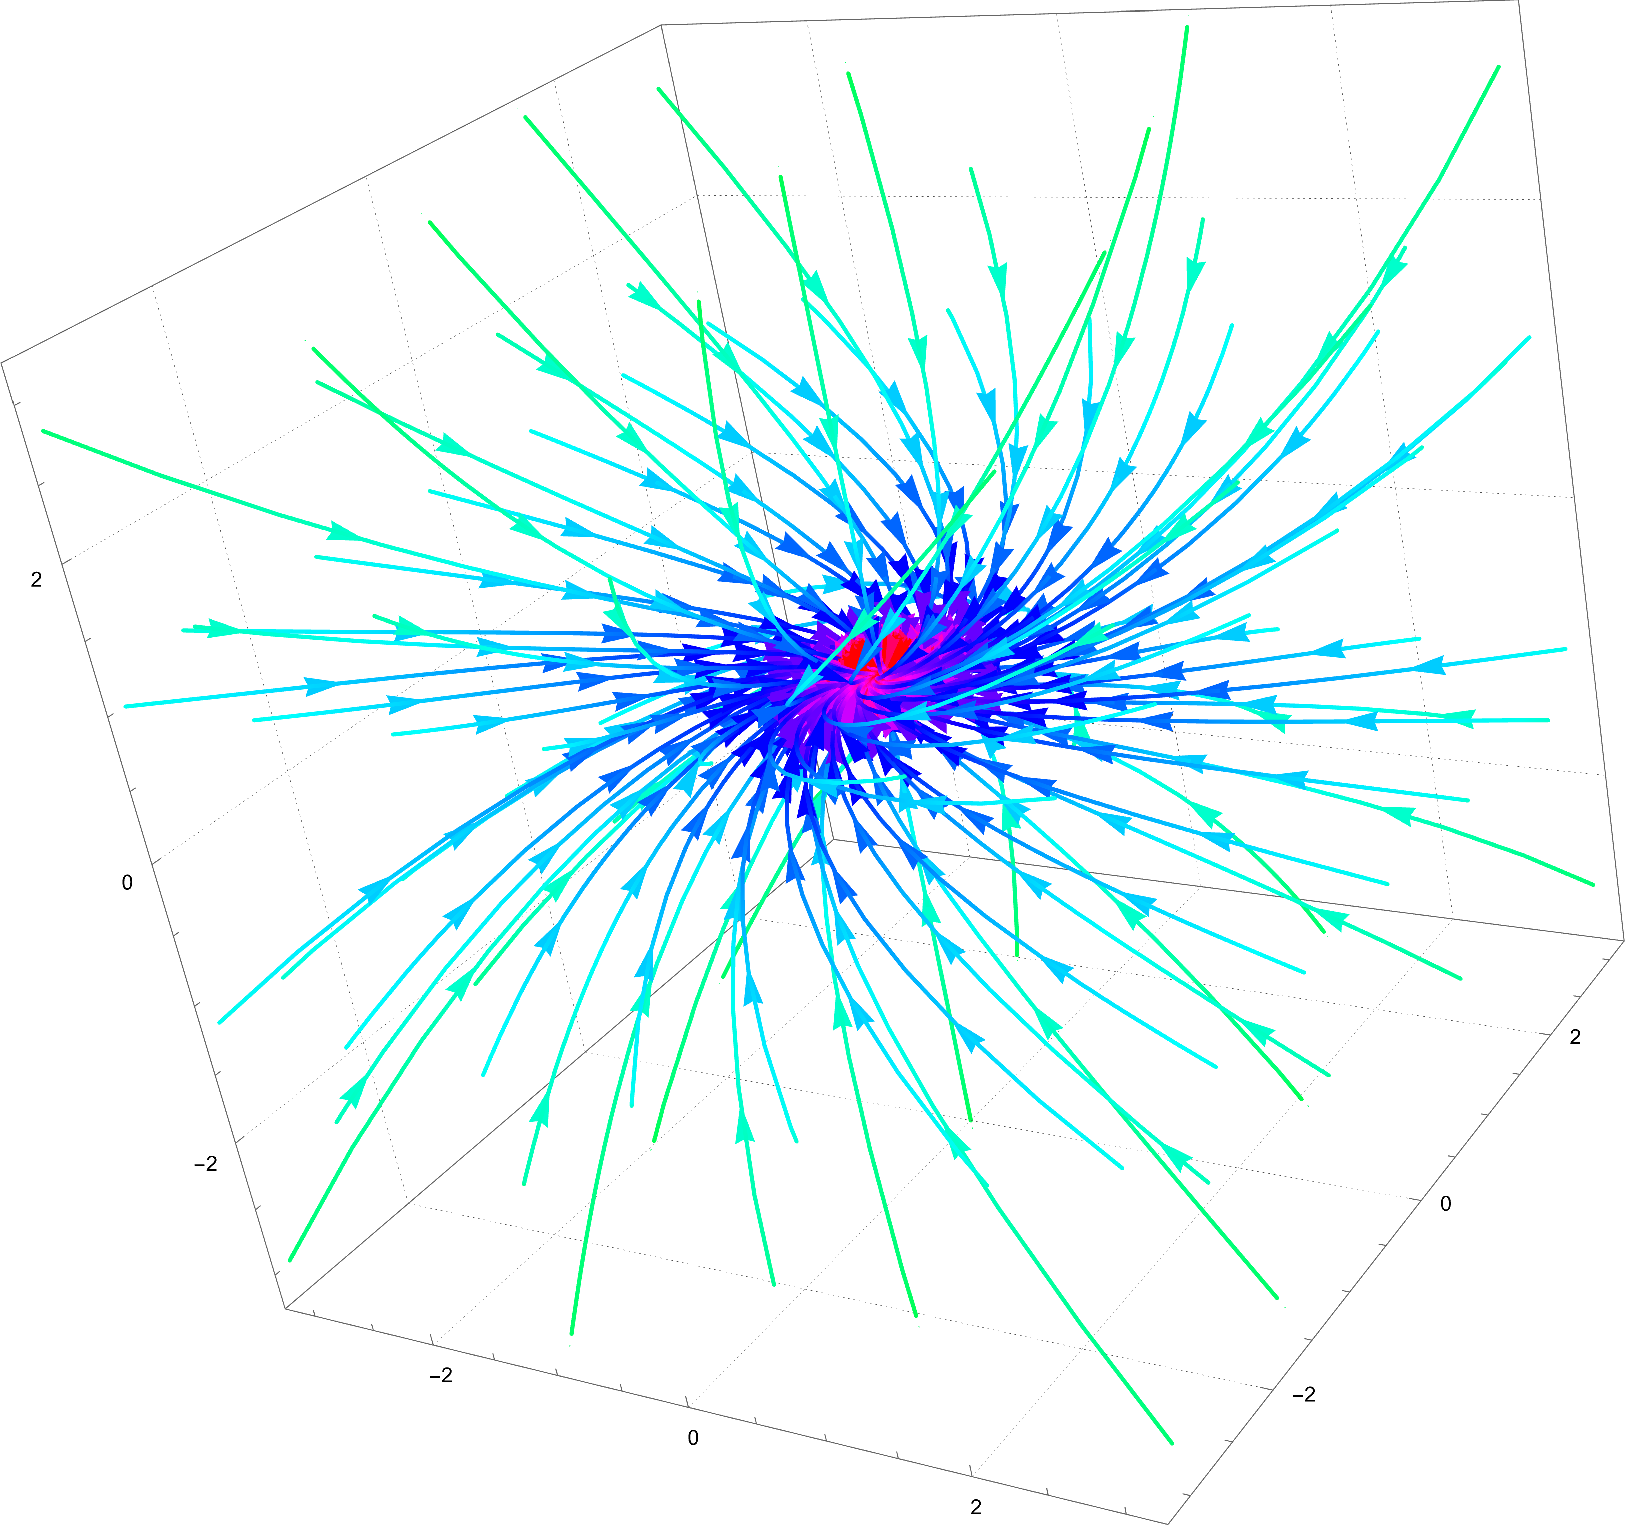
\includegraphics[width=0.5\textwidth]{images/hw_8/case_4.pdf}
\end{figure}

\textbf{Випадок 5.} $\lambda_1 = \lambda_2^*, \; \text{Re}(\lambda_1)<0, \; \text{Re}(\lambda_1)<\lambda_3<0$. Формула знову така сама, але фазовий портрет виглядає зовсім інакше (див. рис. нижче): тут траєкторії ``закручуються'' над і під нашою точкою, що достатньо цікаво. Проте, я не дуже зрозумів, як це побачити з рівняння :)
\begin{figure}[H]
    \centering
    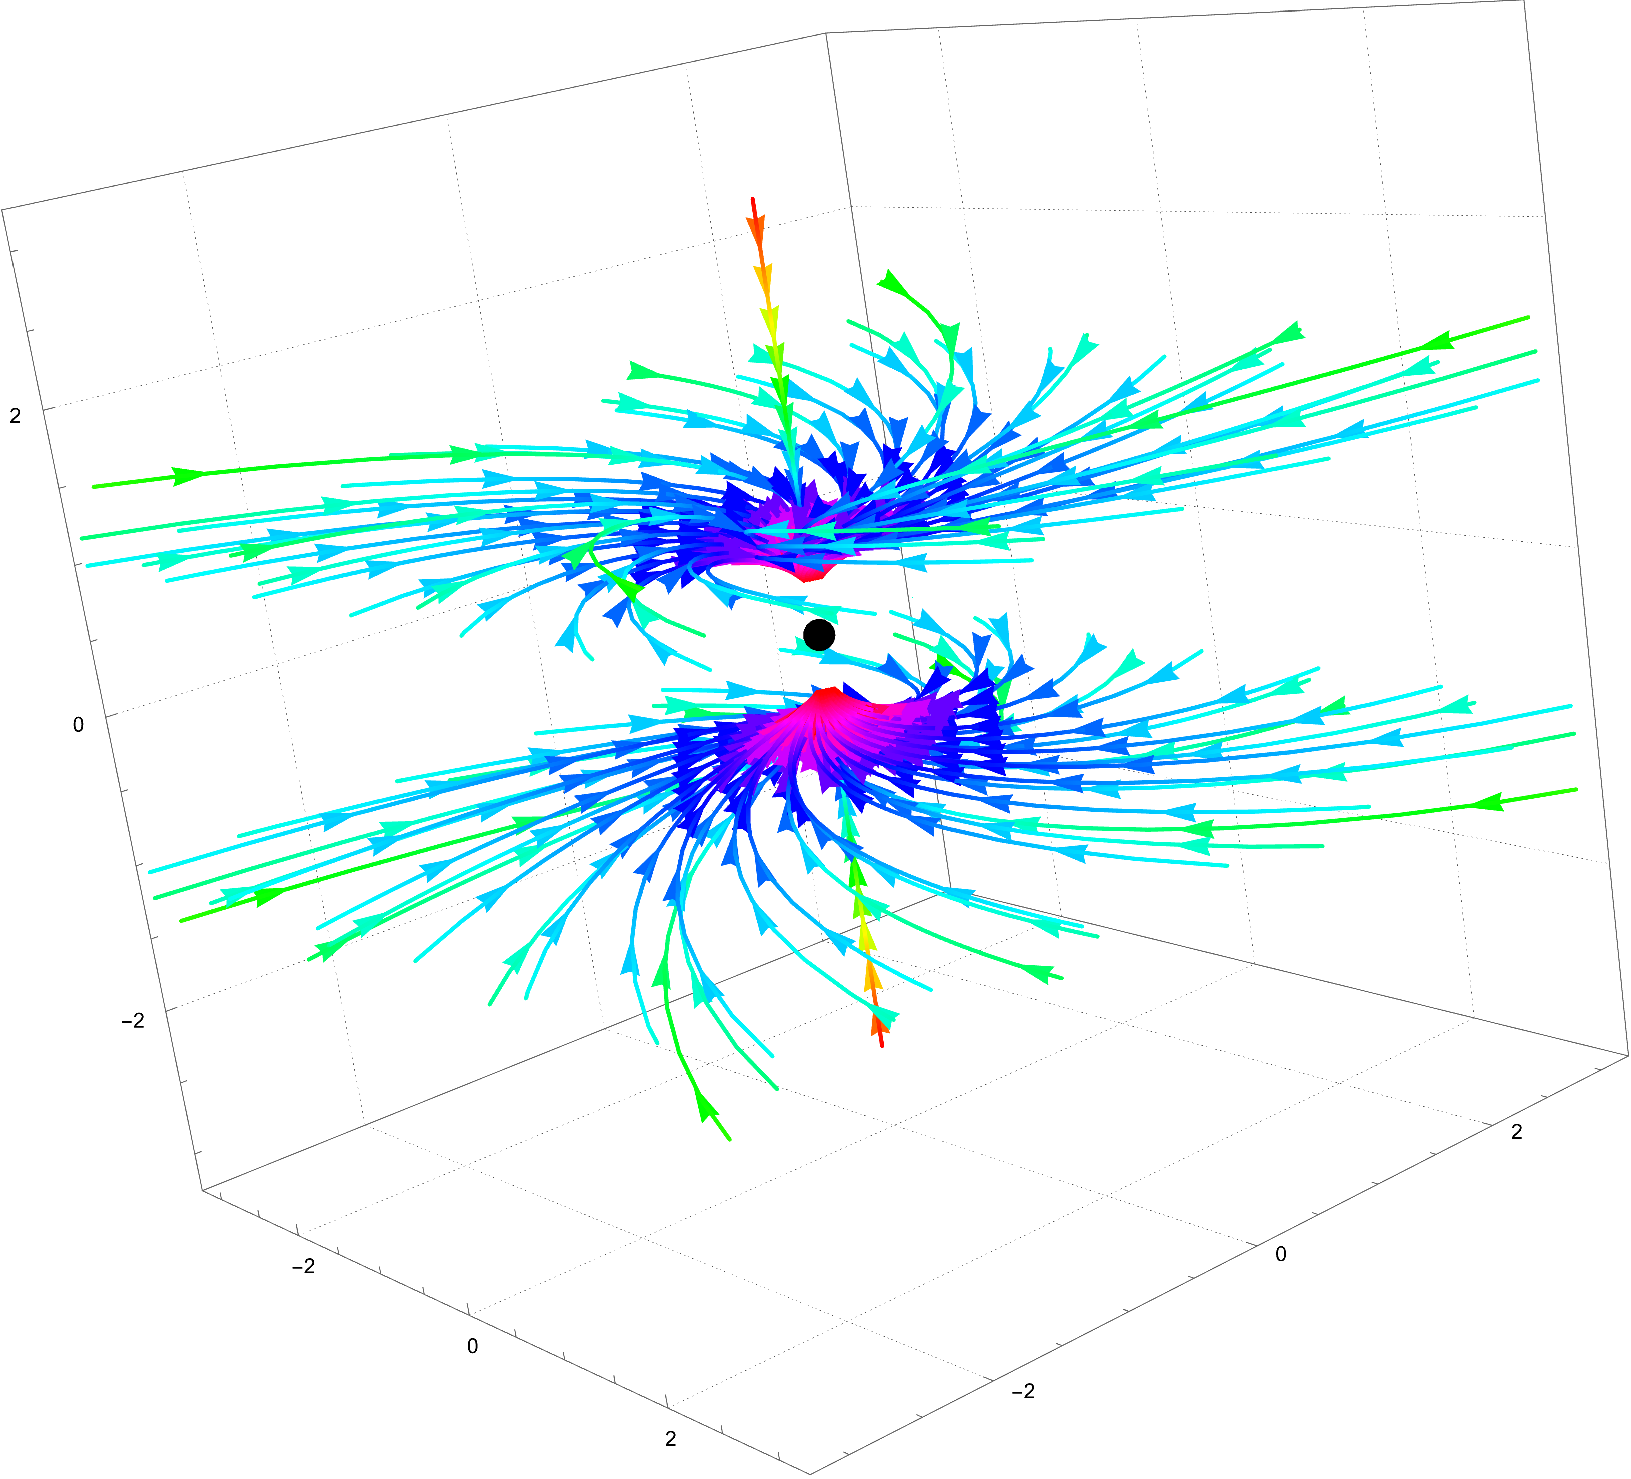
\includegraphics[width=0.5\textwidth]{images/hw_8/case_5.pdf}
\end{figure}

\end{document}
